\documentclass{article}\usepackage{graphicx, color}
%% maxwidth is the original width if it is less than linewidth
%% otherwise use linewidth (to make sure the graphics do not exceed the margin)
\makeatletter
\def\maxwidth{ %
  \ifdim\Gin@nat@width>\linewidth
    \linewidth
  \else
    \Gin@nat@width
  \fi
}
\makeatother

\IfFileExists{upquote.sty}{\usepackage{upquote}}{}
\definecolor{fgcolor}{rgb}{0.2, 0.2, 0.2}
\newcommand{\hlnumber}[1]{\textcolor[rgb]{0,0,0}{#1}}%
\newcommand{\hlfunctioncall}[1]{\textcolor[rgb]{0.501960784313725,0,0.329411764705882}{\textbf{#1}}}%
\newcommand{\hlstring}[1]{\textcolor[rgb]{0.6,0.6,1}{#1}}%
\newcommand{\hlkeyword}[1]{\textcolor[rgb]{0,0,0}{\textbf{#1}}}%
\newcommand{\hlargument}[1]{\textcolor[rgb]{0.690196078431373,0.250980392156863,0.0196078431372549}{#1}}%
\newcommand{\hlcomment}[1]{\textcolor[rgb]{0.180392156862745,0.6,0.341176470588235}{#1}}%
\newcommand{\hlroxygencomment}[1]{\textcolor[rgb]{0.43921568627451,0.47843137254902,0.701960784313725}{#1}}%
\newcommand{\hlformalargs}[1]{\textcolor[rgb]{0.690196078431373,0.250980392156863,0.0196078431372549}{#1}}%
\newcommand{\hleqformalargs}[1]{\textcolor[rgb]{0.690196078431373,0.250980392156863,0.0196078431372549}{#1}}%
\newcommand{\hlassignement}[1]{\textcolor[rgb]{0,0,0}{\textbf{#1}}}%
\newcommand{\hlpackage}[1]{\textcolor[rgb]{0.588235294117647,0.709803921568627,0.145098039215686}{#1}}%
\newcommand{\hlslot}[1]{\textit{#1}}%
\newcommand{\hlsymbol}[1]{\textcolor[rgb]{0,0,0}{#1}}%
\newcommand{\hlprompt}[1]{\textcolor[rgb]{0.2,0.2,0.2}{#1}}%

\usepackage{framed}
\makeatletter
\newenvironment{kframe}{%
 \def\at@end@of@kframe{}%
 \ifinner\ifhmode%
  \def\at@end@of@kframe{\end{minipage}}%
  \begin{minipage}{\columnwidth}%
 \fi\fi%
 \def\FrameCommand##1{\hskip\@totalleftmargin \hskip-\fboxsep
 \colorbox{shadecolor}{##1}\hskip-\fboxsep
     % There is no \\@totalrightmargin, so:
     \hskip-\linewidth \hskip-\@totalleftmargin \hskip\columnwidth}%
 \MakeFramed {\advance\hsize-\width
   \@totalleftmargin\z@ \linewidth\hsize
   \@setminipage}}%
 {\par\unskip\endMakeFramed%
 \at@end@of@kframe}
\makeatother

\definecolor{shadecolor}{rgb}{.97, .97, .97}
\definecolor{messagecolor}{rgb}{0, 0, 0}
\definecolor{warningcolor}{rgb}{1, 0, 1}
\definecolor{errorcolor}{rgb}{1, 0, 0}
\newenvironment{knitrout}{}{} % an empty environment to be redefined in TeX

\usepackage{alltt}
\usepackage[round]{natbib}
\usepackage{caption, amsmath, graphicx, setspace, multirow, color, hyperref, array}

\newcolumntype{x}[1]{%
>{\centering\hspace{0pt}}p{#1}}%

\defcitealias{Netherlands2004}{Netherlands, 2004}
\defcitealias{UNDESA2012}{United Nations, 2012}
\title{A Hedonic Price Analysis of Traffic Noise in the Twin Cities Housing Market}
\date{\today}

\doublespacing
\begin{document}
\maketitle
\begin{singlespace}
\begin{abstract}
One consequence of the expanding road network and its associated traffic is increased levels of traffic noise.  While the hedonic literature has consistently shown a negative effect of this phenomenon on the real estate market, the relationship between housing prices and automobile traffic noise has rarely been explored at landscape level, especially in the United States. Here, we show this relationship by modeling the propagation of traffic noise over the landscape and by analyzing the extent of its impact on single-family home transactions in the urban area surrounding St. Paul, Minnesota using spatially explicit local regression techniques. Our estimate of the negative relationship between traffic noise levels and house prices is smaller in magnitude than most of the relevant published literature. We find no evidence that the effect of traffic noise varies significantly by geography, nor by traffic noise levels.  We find significant differences in the impact of traffic noise before and after the economic recession of 2008-09. Our results suggest that an increase in traffic noise of one decibel decreases house prices by an average of 0.19 percent before September 2008, and an average of 0.37 percent after September 2008.
\end{abstract}
\end{singlespace}

\section{Introduction and Past Research}\label{sec:lit}
Prolonged exposure to traffic noise affects people in a number of ways, ranging from simple annoyance \citep{Miedema2001, Ouis2001, Ohrstrom2007, DeKluizenaar2013, Weinhold2013}, to sleep disturbance \citepalias{Netherlands2004}, to increasing risk for stroke \citep{Sorensen2011}, hypertension \citep{Jarup2008, Bodin2009}, myocardial infarction \citep{Babisch2005}, and overall quality of life \citep{Shepherd2013}. The noise level at which such effects are observed does not have to be high.  It has been shown that people exposed to traffic noise with a 24-hour average of 55 decibels (dBA) are found to be at a higher risk for hypertension \citep{Barregard2009, Bodin2009}, and those exposed to 60 dBA or greater are found to be at a higher risk for stroke \citep{Sorensen2011}.  

Automobiles are already perhaps the greatest source of noise in residential neighborhoods \citep{Barber2010} and traffic noise was estimated to cause around three billion dollars worth of external damage to the United States economy alone in 1991 \citep{Delucchi1998}. Traffic noise and its attendent problems are greater now than they were in the 1990s and predicted to worsen in the future \citep{Goines2007}.  With the exception of a slight dip during the economic recession in the late 2000s, the number of vehicle miles traveled in the United States has steadily increased for the past 50 years.\footnote{\url{http://www.fhwa.dot.gov/policyinformation/statistics/2011/pdf/rc1c.pdf}} Globally, \citet{Dargay2007} predict the number of personal vehicles to grow from roughly 800 million in 2002 to over two billion units by 2030. Additionally, the global trend of increased urbanization is expected to continue, with the proportion of the population living in cities growing from roughly half now to over two-thirds by the middle of the century \citepalias{UNDESA2012}. 

Policies at the local, state, and federal level can influence the level and effect of traffic noise. For instance, the US Federal Highway Admistration reports that 47 states have constructed noise barriers to reduce noise propagation, spending over a half a billion dollars from 2008-2010 \citep{USFHA2012}. The efficiency of such projects requires an understanding of the economic cost of traffic noise. 

One way to estimate some of the costs of traffic noise (and therefore the economic benefits of policies that reduce noise) is through hedonic regression, examining the relationship between house prices and noise levels. \citet{Nelson1982} was the first to review some of the earliest noise hedonic work in the United States and Canada. The review of roughly ten studies found an average estimated impact of traffic noise to be a reduction in house prices of approximately 0.4 percent per additional decibel. More recently, \citet{Nelson2008} notes that many of these early studies \citep[such as][]{Gamble1974, Langley1976} are plagued by issues of small sample sizes (in the hundreds) and limited spatial extents (one or a handful of cities). 

Reviews of the research by \citet{Bateman2001} found that the negative effect of traffic noise on house prices ranged from 0.08 to 2.22 percent per decibel with a mean around 0.55 percent per decibel, while \citet{Navrud2002} found an average decrease of 0.64 percent per decibel. However, much of the research in these reviews and subsequent work has tended to focus on the European experience with noise, especially the United Kingdom \citep{Day2007, Blanco2011}, Sweden \citep{Wilhelmsson2000, Andersson2010}, Switzerland \citep{Baranzini2010}, Spain \citep{MarmolejoDuarteCarlos;GonzalezTamez2009}, Netherlands \citep{Theebe2004a}, and Germany \citep{Brandt2011}. 

Instead of focusing on the impact of automobile traffic, work in the United States has instead tended to concentrate on noise from airports \citep{Espey2000, McMillen2004, Cohen2008a} or indirect effects of traffic noise, such as proximity to highways \citep{Matthews2007, Chernobai2009, Li2012}, or traffic counts \citep{HughesJr.1992, Larsen2012}. One exception is \citet{Cheng2008}, which, using micro data in Louisville, TN during 2007, finds that an additional decibel of traffic noise reduced house prices by 0.34 percent. However, this research is based on less than a thousand transactions.

\citet{Delucchi1998} used an estimate of 0.85 percent reduction in house prices per additional decibel of traffic noise in their cost-benefit analysis of traffic noise. While their preferred estimate of the total damage cost to the United States in 1991 is \$3 billion, they report a possible range of less than \$100 million to over \$40 billion due to uncertainty surrounding the degree of noise propagation over space in the urban built environment and the effect of noise on house prices. Indeed, one of the main conclusions of the \citet{Delucchi1998} is that more research should be done to better understand the impact of noise on house prices and that better noise data are needed for such work to occur. 

One major reason for the thinness of the scholarly literature on this topic in the US lies in the difficulty of modeling traffic noise propagation over the landscape. To properly analyze the spatial association between real estate prices and exposure to traffic noise at a landscape level, it is necessary to create a noise surface map at sufficiently detailed spatial resolution to account for the complex and heterogeneous interaction between the noise source and the resistance of the landscape to noise propagation.  Implementing such a model can be very difficult.  For one thing, the data needed for the model is very extensive and may not even be readily available (e.g., building footprint and height data).  Furthermore, it is computationally very intensive. Fortunately, recent developments in Geographic Information Systems and distributive computing have reduced these difficulties, making it much easier to create a noise surface map at landscape level.  

In this paper, we seek to contribute to the noise hedonic literature by examining the relationship between single family home prices from 2005 to 2010 and variation in road traffic noise exposure in the St.\ Paul, Minnesota urban area. Our work makes three contributions to the field. First, we utilize new estimates of traffic noise that has never before been used in the hedonic literature. The noise propagation model estimates traffic noise levels at a high spatial resolution (10m x 10m) while also incorporating the effects of nearby buildings and landcover. We also construct a flexible hedonic model that allows for a non-stationary relationship between house prices and our explanatory variables over geography and time. Such Locally Weighted Regression (LWR) models have become increasingly common in published work \citep[see][]{MarmolejoDuarteCarlos;GonzalezTamez2009, Carruthers2010, Sunding2010, Nappi-Choulet2011} and have been shown to be more accurate than other spatial econometric models under common circumstances \citep{McMillen2012}. Contrary to previous work \citep{MarmolejoDuarteCarlos;GonzalezTamez2009}, we find that while the impact of other important control variables in the hedonic function vary over space, the impact of traffic noise does not. Lastly, we present the first estimates of the implicit price of traffic noise after the Great Recession and the housing bubble collapse.

\section{Data}
The 2010 US Census lists the population of the Twin Cities Metropolitan Region (Minneapolis and St. Paul and their surrounding areas)  as almost 3 million residents spread over seven counties. This study examines single family residential home transactions in the Census-defined urban areas of three of the seven counties: Dakota, Ramsey and Washington County (see Figure \ref{fig:overview}). We obtained data from approximately forty thousand sales transactions between 2005 and 2010 (n=42,095) from the 2010 MetroGIS Regional Parcel Dataset published by the Metropolitan Council. Figure \ref{fig:overview} shows an overview of the study area as well as the spatial distribution of the house sales prices. In addition to the geographic location and date of the house sale, we collected or calculated structural and locational variables commonly used in the hedonic literature. Table \ref{tab:sumStats} provides a brief description of the variables in our data and some basic summary statistics. Table \ref{tab:cor} shows a simple correlation matrix of the quantitative variables.

\begin{figure}
\makebox[\textwidth][c]{\includegraphics[width = 1.2\textwidth]{../graphs/StudyArea_SaleValueDistribution}}
\caption{This figure shows the spatial extent of our study area as well as the significant spatial variation in single family house sales prices.}\label{fig:overview}
\end{figure}

\begin{table}[htb]
\caption{Variable Description and Summary Statistics}\label{tab:sumStats}
\makebox[\linewidth][c]{
\small
\begin{tabular}{lrrrrrrr}
  
 & min & 25\% & 50\% & mean & 75\% & max & st. dev. \\ 
  \hline
  Sale Price (thousands \$) & 98.8 & 195.0 & 241.0 & 265.5 & 314.9 & 675.0 & 102.8 \\ 
  House Size (feet$^2$) & 390 & 1158 & 1628 & 1750 & 2188 & 4000 & 704 \\ 
  Lot Size (acres) & 0.02 & 0.17 & 0.25 & 0.25 & 0.31 & 0.60 & 0.11 \\ 
  Owner Occupancy (no = 0, yes = 1) & 0.0 & 1.0 & 1.0 & 0.8 & 1.0 & 1.0 & 0.4 \\ 
  Year of House Construction & 1850 & 1950 & 1973 & 1967 & 1993 & 2010 & 32 \\ 
  Traffic Noise (dB) & 25.1 & 50.5 & 55.3 & 56.4 & 62.2 & 91.5 & 8.8 \\ 
  Median Income in Census Tract (thousands \$) & 13.9 & 54.6 & 69.1 & 72.6 & 89.7 & 143.3 & 23.6 \\ 
  Average 3rd Grade Standardized Test Scores & 335.6 & 359.8 & 365.4 & 364.5 & 370.4 & 551.7 & 10.6 \\ 
  Distance to Central Business District (km) & 1.1 & 6.8 & 13.2 & 14.7 & 21.8 & 37.1 & 8.9 \\ 
  Distance to nearest Park (km) & 0.0 & 1.1 & 2.2 & 2.6 & 3.8 & 9.7 & 1.9 \\ 
  Distance to nearest Lake (km) & 0.0 & 0.4 & 0.8 & 0.9 & 1.3 & 4.4 & 0.7 \\ 
  Distance to nearest Shopping Center (km) & 0.0 & 0.9 & 1.5 & 1.9 & 2.3 & 10.8 & 1.6 \\ 
   \hline
\end{tabular}
}
\end{table}

\begin{table}
\caption{Matrix of Pearson Correlation Coefficients for Quantitative Variables}\label{tab:cor}
%\includegraphics[width = \textwidth]{../graphs/CorrelationMatrix}
\begin{center}
\small
\tabcolsep=0.05cm
\begin{tabular}{lrrrrrrrrrrr}
  \hline
 & \multicolumn{1}{x{.35in}}{Price} & \multicolumn{1}{x{.38in}}{House} & \multicolumn{1}{x{.35in}}{Lot} & 
 \multicolumn{1}{x{.35in}}{Built} & \multicolumn{1}{x{.35in}}{Noise} & \multicolumn{1}{x{.35in}}{Inc.} & 
 \multicolumn{1}{x{.35in}}{Test} & \multicolumn{1}{x{.35in}}{CBD} & \multicolumn{1}{x{.35in}}{Park} & \multicolumn{1}{x{.35in}}{Lake} & \multicolumn{1}{x{.35in}}{Shop} \tabularnewline 
  \hline
ln Sale Price & 1 &  &  &  &  &  &  &  &  &  &  \tabularnewline 
  House Size & 0.74 & 1 &  &  &  &  &  &  &  &  &  \tabularnewline 
  Lot Size & 0.40 & 0.45 & 1 &  &  &  &  &  &  &  &  \tabularnewline 
  Year Built & 0.49 & 0.52 & 0.47 & 1 &  &  &  &  &  &  &  \tabularnewline 
  Noise & -0.12 & -0.07 & 0.00 & -0.19 & 1 &  &  &  &  &  &  \tabularnewline 
  Income & 0.55 & 0.50 & 0.41 & 0.57 & -0.18 & 1 &  &  &  &  &  \tabularnewline
  Elem. Test Scores & 0.33 & 0.28 & 0.29 & 0.34 & -0.04 & 0.44 & 1 &  &  &  &  \tabularnewline 
  Distance to CBD & 0.35 & 0.45 & 0.43 & 0.58 & -0.04 & 0.53 & 0.35 & 1 &  &  &  \tabularnewline
  Distance to Park & 0.27 & 0.28 & 0.22 & 0.42 & -0.13 & 0.38 & 0.22 & 0.57 & 1 &  &  \tabularnewline
  Distance to Lake & -0.05 & -0.10 & -0.25 & -0.17 & -0.03 & -0.12 & -0.10 & -0.09 & 0.20 & 1 &  \tabularnewline
  Distance to Shop & 0.28 & 0.27 & 0.15 & 0.37 & -0.19 & 0.36 & 0.18 & 0.46 & 0.38 & 0.15 & 1 \tabularnewline
   \hline
\end{tabular}
\end{center} 
\end{table}


\subsection{Structural Attributes}
According to a review by \cite{Wilhelmsson2000}, the most common structural attributes included in real-estate hedonic pricing studies are living area, number of bathrooms, age, garage and lot size.  Although the 2010 MetroGIS Regional Parcel Dataset includes structural data on living area, age, garage presence, lot size and owner occupancy for every transaction, we have variables for the number of bedrooms, bathrooms, and size of the garage only for those house sales in one county. We feel confident in our results even without these independent variables for most of our study data because sensitivity analysis conducted in areas with the additional structural variables revealed very similar estimates when the variables were included and excluded. These results are in section \ref{Discussion} of the the paper. Additionally, other hedonic work has been published using a similar set of explanatory variables in this area, see for instance, \citet{Sander2009b}.

\subsection{Noise Data}
Insert noise data description and methodology here. \citet{Nega2012}
To determine the relationship between real estate price and road traffic noise levels, we first created a traffic noise exposure surface for the entire Twin Cities Metro Region (TCMR) by calculating the propagation of traffic noise over the landscape using the FHWA (Federal Highway Authority) 1978 standard \citep{Barry1978}. Following \citet{Barry1978}, the traffic noise level at any given location on the landscape is given by: 
\begin{eqnarray}\label{eq:noise}
L_{EQ}(i) &=& \bar{L}_0(i) + 0.115 \sigma _i^2 + 10 log \frac{N_i \pi D_0}{T*S_i} + 10 log \left[ \frac{D_0}{D}\right]^{1 + \alpha}  \nonumber \\
&& + 10 log \left( \frac{\psi _{\alpha (\phi _1, \phi _2)}}{\pi}\right) + \Delta _{gradient} + \Delta _{shielding}
\end{eqnarray}
where $L_{EQ}(i)$ is A-weighted hourly energy equivalent noise level in dBA, which is calculated for each class $i$ of vehicle (automobile and trucks); $\bar{L}_0(i)$ is the mean Sound Pressure Level (SPL) at the reference distance for class $i$; $\sigma _i$ is the standard deviation of the SPL for each class of vehicle; $N_i$ is the number of vehicles of the $i^{th}$ class passing during the relevant hour; $D_0$ is the reference distance (usually 15 m); $D$ is the perpendicular distance from the road center line to the receiver; $\alpha$ is a site parameter (soft and hard surface), $0 < \alpha < 1$; $S_i$ is the mean speed of the $i^{th}$ class; $T$ is the duration, usually 1 hour; $\phi _1$ and $\phi _2$ are the angles from the perpendicular of the limits of the observer's view of a section of the road. They are used to account for only the energy coming from a portion of the roadway; $\Delta _{gradient}$ is an adjustment for road surface gradient; $\Delta _{shielding}$ is a shielding adjustment (land cover, buildings, noise barriers).

To calculate the traffic noise map for the region using the above model, several data sources were used. A 2007 road centerline and the associated traffic characteristics (volume and proportion of trucks and vehicles) for the region were obtained from the Minnesota Department of Transportation (MNDoT). We converted the posted speed of each road into a GIS layer. For all roads without recorded traffic volume (i.e., residential), we assigned 100 vehicles/day as a minimum estimate. This estimate was based on factors identified in the literature as important for estimating traffic volume, such as census data on commuting population, tract area, the size of a standard street block, and road type \citep{Cheng1992, Fricker1986}.\footnote{In order to assess the sensitivity of our results to our estimate of traffic volume for local roads, we conducted a sensitivity analysis by running the model using 200 and 300 vehicles/day for one of the counties that make up the TCMR. With the exception of a few areas in the rural part of the county, there was less than 0.05 dBA difference at 30 m from the road centerline, suggesting that the estimated values are not sensitive to the traffic volume variations used for the sensitivity analysis.}

Data on traffic volume and the proportion of trucks and vehicles on each segment of the road were averaged over a 24-hour period, making it impossible to account for a day and night time variation in traffic noise. Following \citet{Arditi2007}, we divided the total traffic volume into day and nighttime periods by assuming that 80 percent of vehicles and 65 percent of trucks are driven during the daytime (6am–10pm) and 35 percent of trucks and 20 percent of vehicles are driven during the nighttime (10pm-6am). Values for ground absorption were chosen by assuming that all road surfaces consisted of impervious bitumen. For computational simplicity, we created the road surface gradient by re-sampling U.S. Geological Survey 30 m resolution Digital Elevation Model (DEM) to 100 m resolution. 

We used three data sources for the shielding adjustment: buildings, foliage, and noise barriers. We extracted the perimeter and height of 818,500 buildings using aerial photography and LiDAR data. For the areas where LiDAR data are available, we used LiDAR Analyst$^{TM}$ software to extract buildings’ footprints. For the areas of the region where only aerial photos are available, we used Feature Analyst$^{TM}$ software to extract building footprints. For measurements extracted using aerial photography, height was determined using a combination of parcel data and field measurements. 

The locations chosen for the traffic noise levels were the 818,500 buildings in the TCMR. Thus, we used the perimeter and height of these buildings to account for the shielding effect of buildings. To account for foliage shielding (and to make the computation manageable), we assumed that only forest patches that are at least 10 m high and have an area greater than 10,000 m$^2$ will have a significant effect on noise attenuation. Accordingly, we extracted forest polygons with these characteristics using a combination of year 2005 land use data and 2001 National Land Cover Data (NLCD). To account for noise barrier shielding, we used a noise barrier layer obtained from MNDoT, which contains the locations, width, and height of noise barriers in the region.

We used the SoundPlan$^{TM}$ noise modeling software to implement the model given by Equation \ref{eq:noise}. Predicted traffic noise output is calculated at a grid resolution of 10 m$^2$.\footnote{We conducted a preliminary validation of the model output by comparing it with observed noise levels at 134 locations that were sampled along major highways. For each location, two readings were taken very close to the highway, one between 9am and 10am and another between 1pm and 2pm. The noise level for each location is then determined by averaging the two observed values, and this average is then compared with the predicted noise level. The relationship between the mean observed and predicted noise levels is linear and moderately strong with a correlation of 0.76. It is not surprising that the relationship is not stronger given the size and complexity of the model. In particular, the traffic volume data that we used for modeling traffic noise propagation is a 24-hour average, which requires more time-interval sampling per location than just the two used in the validation. Still, this preliminary comparison serves as a good indicator of how well this model captures traffic noise levels.} Once the noise surface for the entire region was developed, we extracted the noise surface for the present study area by overlaying the housing parcel boundaries and calculating the maximum noise level within the parcel.

\subsection{Other Locational Attributes}
A common real estate addage states that the three most important real estate attributes are: location, location and location. Knowing where each house is located allows us to also construct a vector of other attributes associated with the sales transaction. For instance, using GIS software we are able to calculate the Euclidean distance to numerous points of interest within the dataset, such as the nearest central business district, shopping centers, parks, and lakes. Additionally, a variable denoting the median household income for the surrounding census tract is created through the use of TIGER shapefiles from the 2010 Census Bureau and data from the 2010 American Community Survey (ACS). Lastly, we associate each transaction with its elementary school and include the average 3rd grade Minnesota Comprehensive Assessment (MCA) score for the local elementary school during the year of purchase.\footnote{Test scores were obtained from the Minnesota Department of Education website. The school district and elementary school attendance boundary spatial information was taken from the Minnesota Geospatial Information Office Clearinghouse Data Catalog.} 

\subsection{Time}
Given that we have data from before and after the recession of 2008-09, we subset the data in Table \ref{tab:SumStatsTime} by year of sale to look for differences over time. In addition to the noticeable decline in nominal sales values, there is also a drop in the number of sales across years. For example, in 2010 there were only 4,206 property sales within the dataset, less than half as many in 2005. While the mean sale price declined from roughly \$280,000 pre-crash to \$230,000 post-crash, most of the structural and neighborhood variables are relatively consistent across years. However, traffic noise displays a noticeable difference in the pre- and post-crash market transactions (the mean drops from 58 dB to 52 dB). 

\begin{table}
\caption{Mean Variable Values Across Time}\label{tab:SumStatsTime}
\includegraphics[width = \textwidth]{../graphs/DescriptiveStatsByYear}
\end{table}

\section{Basic Econometric Model}\label{basicModel}
Consistent with past research, this study implements a semi-logarithmic hedonic pricing model. Our aim is to estimate the marginal willingness to pay for different attributes, in particular changes in the traffic noise associated with the house. Equation~\eqref{eq:model} expresses the basic hedonic model.
\begin{equation}\label{eq:model}	
ln \textrm{ Sale Price}_i = \beta _0 + \beta _1 \textrm{Noise}_i+ \beta _2 S_i+ \beta _3 N_i + \beta _4 T_i + \textrm{error}_i
\end{equation}
Where Noise$_i$ is the noise level for house $i$, $S_i$ is a vector of the house's structural attributes, $N_i$ is a vector of the neighborhood attributes, and $T_i$ is a vector of year fixed effects. We can interpret the regression model coefficients as the price semi-elasticities of the underlying attributes. For instance, we can interpret the coefficient on noise as the percentage increase in price for a one decibel increase in the traffic noise associated with the transaction in our dataset. 

\begin{table}
\caption{Basic Regression Results- Dependent Variable = $ln$ Sale Price}\label{tab:globalRegression}

\makebox[\textwidth][c]{\includegraphics[width = 1.3\textwidth]{../graphs/GlobalRegression}}
\end{table}

Standard urban economic theory\footnote{Cite Muth, Mills, etc. here.} predicts that the price of land will vary over space within our dataset to account for locational amenities. As such, we add interaction terms between lot size and distance to the nearest central business district to account for spatial variation in the price of land. The first column in Table \ref{tab:globalRegression} shows the results of this regression. The negative coefficient of -0.0027 on the noise variable (a one dB increase in noise decreases house price by 0.27 percent) is in line with the estimates described earlier in the literature. The significant coefficients on the lot size interaction terms suggest that the value of land varies over space. The significant coefficients on the non-linear interaction terms suggests that the nature of the spatial variation in the value of land may be complex.

Table \ref{tab:globalRegression} also attempts to begin to understand how the economic recession may have influenced the hedonic function in our study area. The other columns in the table show the regression output from separating the data into sales before and after September of 2008 (the month that the US Federal government took over Fannie Mae and Freddie Mac, Lehman Brothers filed for bankruptcy, and the American International Group (AIG) narrowly avoided bankruptcy only through a \$85 billion loan from the US Federal government).\footnote{\url{http://www.federalreserve.gov/newsevents/press/other/20080916a.htm}} The coefficients for some of the hedonic variables of interest (noise, schools, land, for instance) appear different across the two time periods.

Taken in aggregate, the results in Table \ref{tab:globalRegression} suggest that the hedonic price function may vary over space and time. While methods exist for parameterizing this variation \citep[such as spatial expansion as suggested by][]{Casetti1972}, we have no a priori knowledge of how to parameterize the variation over space and time. As such, we turn to a semi-parametric form of hedonic regression, a flexible modeling approach which lets the data reveal how relationships vary, rather than specifying them beforehand.

\section{Locally Weighted Regression Model}
Locally Weighted Regression (LWR) techniques (also known as Geographically Weighted Regression) are described in detail by \citet{Cleveland1988}, \citet{Brunsdon1998b}, \citet{Fotheringham2002}, and others. It is a weighted least squares methodology in which regression coefficients are estimated over space as a function of the local data as described in Equation~\eqref{eq:LWRbeta},
\begin{equation}\label{eq:LWRbeta}
\hat{\beta}_i = (X'W_iX)^{-1}X'W_iY,
\end{equation}
where X is a $n \times m$ matrix of independent variables, $W_i$ is the $n \times n$ weights matrix, and Y is the $n \times 1$ vector of dependent variable values. The weights matrix, $W_i$ is a diagonal matrix where element $w_{jj}$ denotes the weight that the $j^{th}$ data point will receive in the regression coefficients estimated at location $i$ in the dataset. We employ a bi-square weights function and a k-nearest neighbor bandwidth approach as described in equation~\eqref{eq:weights}, 
\begin{equation}\label{eq:weights}
w_{jj}=\left[1-\left(\frac{d_{ij}}{d_{k}}\right)^2 \right]^2 \textrm{ if  }d_{ij}<d_{ik}\textrm{, otherwise = 0},
\end{equation}
where $d_{ij}$ denotes the distance between observations $i$ and $j$, and $d_{ik}$ is the distance from observation $i$ to the $k^{th}$ nearest observation. This function assigns weights close to 1 for data points near observation $i$, weights positive but closer to zero for observations farther away, and zero for all $n-k$ observations farther away than the $k^{th}$ nearest observation. 
We estimate LWR coefficients using bandwidths ranging from as small as 50 observations and as large as 10,000 observations. We choose the LWR bandwidth my minimizing the Generalized Cross Validation score as detailed in equation~\eqref{eq:GCV},
\begin{equation}\label{eq:GCV}
n*\sum_{i=1}^{n}\frac{(y_i-\hat{y}_i)^2}{(n-v_1)^2}, 
\end{equation} 
where $y_i$ is the dependent variable value, $\hat{y}_i$ is the predicted dependent variable value for observation $i$, and $v_1$ is the ``effective number of model parameters.''
$v_1=$tr(\textbf{S}), where the matrix \textbf{S} is the ``hat matrix'' which maps $y$ onto $\hat{y}$,
                   \begin{equation*}
                   \hat{y}=\textbf{S}y,
                   \end{equation*}
                   and each row of \textbf{S}, $r_i$ is given by:
                     \begin{equation*}
                   r_i=X_i(X'W_iX)^{-1}X'W_i.
                   \end{equation*}                
\section{Results}
Similar to the basic econometric model described in Section \ref{basicModel}, the LWR model estimates the logged sales price of a house as a function of structural, locational and temporal variables. In order to account for changing market conditions over time in our data, when estimating LWR coefficients we use only houses sold within the past 12 months. Thus, the coefficient estimates at a particular house are estimated using data from other sales nearby in both time and geography.

Figure \ref{fig:GCVmodel} shows the relationship between the number of nearest houses receiving positive weights in the Locally Weighted Regression and the Generalized Cross Validation score across three different models. The first model simply uses the basic structural characteristics as the explanatory variables (size of the house in square feet, size of the lot in acres, a categorical variable denoting the architectural style of the house, and whether or not the house is owner-occupied). The second model adds locational variables to the previously described model (test scores at the local elementary school, census tract median income, and distances to the central business district, nearest park, nearest shopping center, and nearest lake). The third model adds city fixed effects. Generally speaking, the third model performs slightly better than the second model, which performs better than the first model. The minimum GCV score is obtained using a bandwidth of 200 nearest houses and Model (3).
\begin{figure}
  \makebox[\textwidth][c]{\includegraphics[width = 1.2\textwidth]{../graphs/GCVbyModel}}
\caption{This figure shows the relationship between bandwidth size and the GCV score for three different Locally Weighted Regression (LWR) models. For comparison, the GCV scores for each model when estimated at a global scale are also shown. Note that the LWR models all have significantly smaller GCV scores than the global models. The minimum GCV score is obtained by LWR Model (3) at a bandwidth of 200 nearest houses.}\label{fig:GCVmodel}
\end{figure}

Figure \ref{fig:GCVmodel} also displays the GCV scores for the three models estimated at the global scale. The GCV scores for the global models follow a similar patter as the LWR models, with Model (3) performing better than Model (2) and Model (1) having the highest GCV score. It is also worth noting that the LWR models have significantly lower GCV scores for a range of bandwidths when compared to the global models. These results suggest that it is important to model our data in a spatially explicit manner. Table \ref{tab:mainresults} displays a summary of the results of LWR Model 3 and a similar regression model run without allowing for spatial variation in the regression coefficients. Again, note that the LWR model yields a substantially smaller GCV score (0.027 vs.\ 0.041).

% latex table generated in R 2.15.2 by xtable 1.7-0 package
% Mon Jun 24 16:36:58 2013

\begin{table}[bp]
\caption{Hedonic Regression Results (dependent variable = $ln(\textrm{Sale Price})$)} \label{tab:mainresults} 
\makebox[\linewidth]{
\small
\begin{tabular}{lrrrrrr} \\
 & \multicolumn{2}{c}{Global Model} & \multicolumn{4}{c}{Locally Weighted Regression Model} \\
 & \multicolumn{1}{c}{$\hat{\beta}$} & \multicolumn{1}{c}{$\hat{\sigma}_{\hat{\beta}}$} & mean $\hat{\beta}$ & \multicolumn{1}{c}{$\sigma_{\hat{\beta}}$} & (5) & (6) \\ 
  \hline
(Intercept) & 8.4E+00 & 1.3E-01 & 2.9E+00 & 1.5E+01 & 0.64 & 0.00 \\ 
  Traffic Noise & -2.6E-03 & 1.6E-04 & -2.5E-03 & 3.0E-03 & 0.47 & 0.67 \\ 
  House Size & 3.0E-04 & 2.7E-06 & 2.6E-04 & 9.1E-05 & 1.00 & 0.00 \\ 
  Lot Size & 2.6E-01 & 1.5E-02 & 4.0E-01 & 3.7E-01 & 0.67 & 0.00 \\ 
  Year of Construction & 1.2E-03 & 6.5E-05 & 4.5E-03 & 5.4E-03 & 0.79 & 0.00 \\ 
  Owner Occupancy & 2.7E-02 & 3.2E-03 & 2.3E-02 & 6.4E-02 & 0.37 & 1.00 \\ 
  Elementary Test Scores & 1.5E-03 & 1.2E-04 & 2.4E-04 & 3.1E-02 & 0.30 & 0.00 \\ 
  Median Income & 3.3E-06 & 7.7E-08 & 9.6E-07 & 8.1E-06 & 0.35 & 0.00 \\ 
  distance to CBD & 1.3E-05 & 6.3E-07 & 1.1E-05 & 1.0E-04 & 0.30 & 0.00 \\ 
  `` nearest Park & -3.7E-07 & 1.1E-06 & -1.6E-05 & 1.3E-04 & 0.32 & 0.00 \\ 
  `` nearest Lake & 2.5E-05 & 2.1E-06 & -2.8E-05 & 1.4E-04 & 0.35 & 0.00 \\ 
  `` nearest Shopping Center & -5.3E-06 & 1.3E-06 & 1.5E-05 & 8.8E-05 & 0.29 & 0.00 \\  
  location of sale & \multicolumn{2}{c}{city fixed effects} & \multicolumn{4}{c}{\footnotesize city fixed effects and nearest 200 sales} \\
  timing of sale & \multicolumn{2}{c}{year fixed effects} & \multicolumn{4}{c}{within last 12 months} \\
 \hline
  GCV score & \multicolumn{2}{c}{0.041} & \multicolumn{2}{c}{0.027}  &  & \\
  Moran's I statistic & \multicolumn{2}{c}{0.199} & \multicolumn{2}{c}{0.012} & & \\
\end{tabular}
}
 \caption*{\footnotesize Column (5) displays the proportion of $\hat{\beta}_{LWR}$ that can reject the null hypthesis of $\beta =0$.\\ Column (6) displays the proportion of Monte Carlo simulations with larger standard deviations of the LWR coefficients than $\sigma_{\hat{\beta}}$}
\end{table}

The first column in Table \ref{tab:mainresults} displays the estimates from a standard semi-log OLS regression with traffice noise, structural characteristics, location-based amenities, and both city and year of sale dummy variables. The coefficient in the second row of the table shows the estimated impact of an additional dB of traffic noise on the natural log of the house sale price to be -.23 percent. This value is within the range of other estimates as described earlier in section \ref{sec:lit}. Coefficients for the dummy variables (on house style, city, and year of sale) are not reported for the sake of brevity, but are available upon request. The second column in the table reports the estimated coefficient standard errors. With the exception of the coefficient on the distance to the nearest park, all reported coefficients are statistically different from zero at conventional levels. 

The third column displays the mean estimated coefficients from the LWR model. In this model coefficients are estimated at each observation within the dataset using the nearest 200 house sales within the past 12 months. The fourth column displays the standard deviation of the estimated coefficients to give a sense of how the coefficients vary when allowed to do so through the use of locally weighted regression techniques.

Column (5) in Table \ref{tab:mainresults} shows the percentage of the local regressions for which the coefficient's p-value is less than 0.1. All regressions contained statistically significant estimates of the impact of increased living space and a majority contained significant estimates for lot size and year of construction. Roughly half of the regressions estimated an impact of traffic noise statistically different from zero, while approximately one-third of the local regressions estimated statistically significant estimates of the locational variables (school test scores, census tract median income, distance to local amenities).

The lack of statistical significance for many of the local regression coefficients could be due to multiple factors. First, because we are estimating local regressions with only the nearest 200 data points, rather than over 30,000 sales as in the global model, we might be estimating the coefficients with less precision and are unable to differentiate the coefficients from zero. Alternatively, the coefficients themselves might vary, sometimes being close to zero and other times not. This variation might be due to random chance (after all, we have estimated tens of thousands of regressions), or it could be the result of true spatial non-stationarity on the part of the coefficients. 

\subsection{Does the Hedonic Function Vary over Space?}
We believe the use of a LWR estimation procedure is appropriate after conducting two different Monte Carlo simulations with the data as described in \citet{Fotheringham2002}. In each simulation we resampled (without replacement) the location of each house in the study and then re-estimated the LWR model with the locationally ``shuffled'' data. In the first simulation we estimated the LWR model using bandwidths ranging from the nearest 50 to 10,000 sales just as before. In 100 consecutive simulations, the smallest Generalized Cross-Validation score was obtained at the largest bandwidth. The smallest of these GCV scores was 0.041, just as was the case with the global (non-LWR) model. In other words, after running thousands of regressions on the shuffled data, we never obtained results anywhere near LWR model with our true locational data. This seems to be strong evidence that the increased ability to predict house prices with a local model is not due to chance. 

In the previous simulation we found that the hedonic regression function indeed exhibits spatial non-stationarity. However, we have not yet established which variables have spatially varying coefficients. In the second simulation, we seek to explore which of the hedonic regression coefficients exhibit spatial non-stationarity. We repeat the Monte Carlo simulation described earlier, but only at the optimal bandwidth calculated in original LWR model and we also kept track of the standard deviation of the estimated LWR coefficients for each variable. The intuition of the simulation is as follows: a variable might truly exert a spatially stationary effect on house prices, but our estimates vary over space due to chance. If this is the case, by shuffling the location of our observations and rerunning the LWR model, we should see a similar dispersion in regression coefficients over space. However, if the coefficient exhibits true spatial non-stationarity, it is unlikely that we will see as large of a standard deviation in the coefficient estimates after having reshuffled the data (because now the houses for which a coefficient exerts a strong effect are now no longer near each other). 

After $M = 100$ iterations of this simulation, the minimum GCV score for these resampled LWR models is 0.060, substantially larger than all models (global and local) with the actual data. The fourth column in Table \ref{tab:mainresults} displays the standard deviations of the LWR regression coefficients obtained with our data. Column (6) displays the proportion of Monte Carlo simulatons that yielded larger standard deviations of LWR coefficient estimates than those shown in column (4). For most variables, we never obtained a larger coefficient standard deviation in the simulation than we obtained from the LWR model with the actual data. However, the values associated with the traffic noise and owner occupancy variables suggest that the variation in LWR coefficients in our data may have been due to random chance. These coefficients may in fact be stationary across the study area, while the other coefficients appear to be non-stationary. Future work may want to estimate a mixed-LWR model in which the coefficients on traffic noise and owner occupancy remain stationary while the other coefficients are allowed to vary over space. See \citet{Fotheringham2002} for a description of a mixed-LWR estimation algorithm. 

Figure \ref{fig:MCsds} visually shows the results presented in column (6) of Table \ref{tab:mainresults} another way. Each subfigure displays the distribution of LWR coefficient standard deviations obtained from the 100 iterations of the Monte Carlo simulation and the standard deviation obtained with the actual data (in red). Note that it is the case that the standard deviations obtained with the actual data are substantially larger than those obtained in the simulation for most of the variables.

\begin{figure}
 \makebox[\textwidth][c]{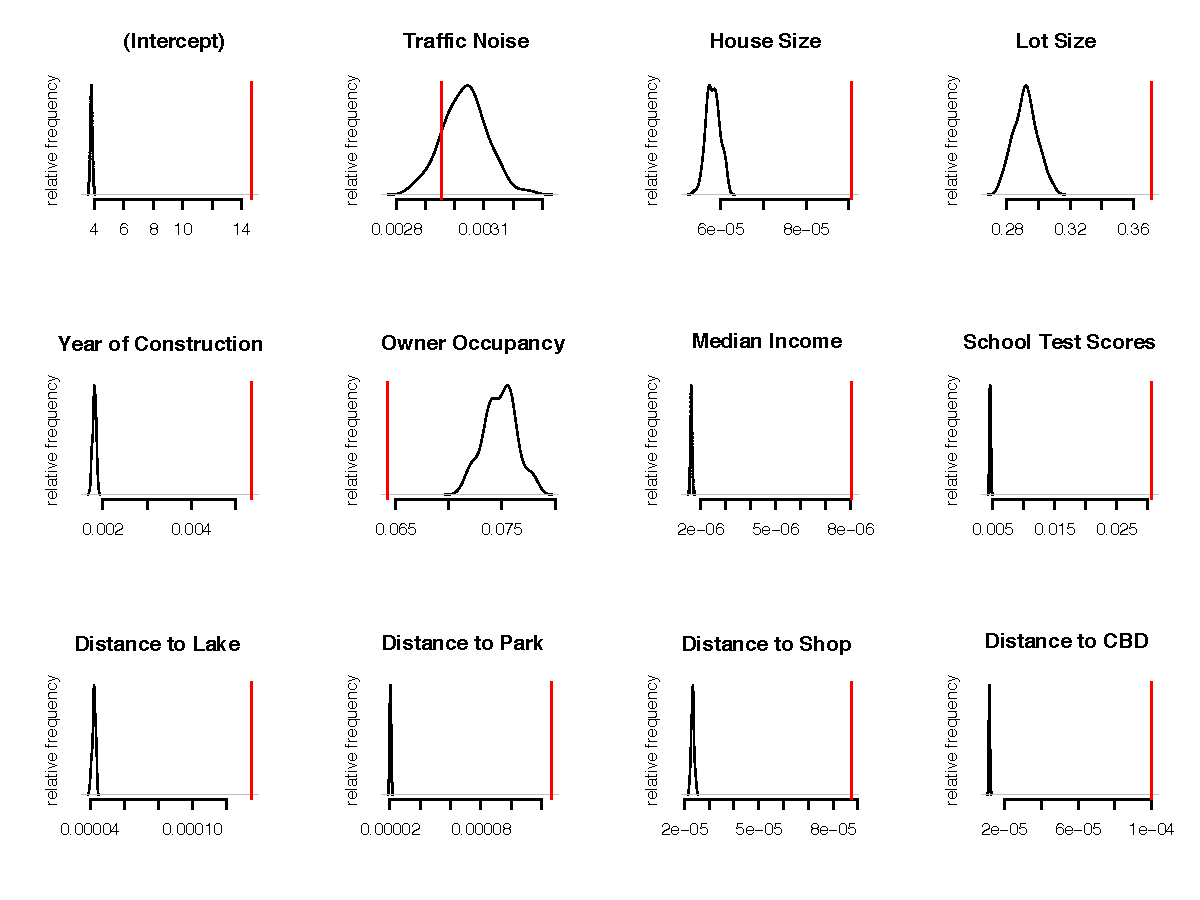
\includegraphics[width=1.2\textwidth]{../graphs/MCsimResultsSDsClean}}
 \caption{Actual LWR Coefficient Standard Deviations \textcolor{red}{(red line)} vs.\ Distribution of Monte Carlo Simulation Standard Deviations by Variable.}\label{fig:MCsds}
\end{figure}
 
In addition to the LWR model with a bandwidth of the nearest 200 houses and a temporal lag of 12 months performing better than other bandwidths and model specifications in terms of the smallest GCV score, it also exhibits far less spatial autocorrelation within the model residuals. We calculate the Moran’s I statistic to be 0.199 for the global model while our prefered LWR specification reduces the Moran's I statistic to 0.012, a nearly twenty-fold reduction. 

\subsection{Does the Implicit Price of Traffic Noise Change over Time?}

Previous research has suggested that the impact of noise can change with time and economic conditions. For instance, \citet{Wilhelmsson2000} found that the traffic noise penalty to be stronger in the 1990s near Stockholm, Sweden compared to the 1980s. \citet{Cohen2009} also found the (airport) noise penalty to be larger in the early 2000s compared to the late 1990s in Atlanta, Georgia. We know that house prices in the United States fell dramatically during and after the Great Recession of 2008-09. We know less about the patterns of change in the hedonic price functions during and after the fall in prices. \citet{Cho2011b} found evidence from hedonic analysis in the Nashville, Tennessee area that consumers' willingness to pay for environmental amenities (such as proximity to open space and water views) decreased during the recession as compared to the previous economic boom. 

In this section we look for evidence of temporal non-stationarity in the hedonic coefficient on traffic noise within our data. Specifically, we create two new variables, ``\texttt{months since September 2008}'' and a dummy variable ``\texttt{post}'' for all sales after September 2008. We then regress our LWR noise coefficients on these two variables and their interaction term as shown in equation \eqref{eq:LWRinteraction}, 
\begin{equation}\label{eq:LWRinteraction}
\hat{\beta}_{LWR} = \alpha _0 + \alpha _1 \texttt{*Month} + \alpha _2  \texttt{*Post} + \alpha _3 \texttt{*Post*Month} + \epsilon.
\end{equation}
The results of this regression will help us understand the patterns of change in the implicit price of traffic noise. In particular, $\alpha_1 \neq 0$ suggests a linear temporal trend in the marginal willingness to pay to avoid traffic noise, while $\alpha_2 \neq 0$ suggests that there was a structural break after September 2008, and $\alpha_3 \neq 0$ will imply a change in the temporal trend after September 2008. The linear regression results presented in Table \ref{tab:betaMAX} show that there is a significant negative shock to the estimated LWR coefficients for traffic noise after September 2008. Additionally, the coefficients also begin to a significant negative trend.
\begin{table}[h]
\caption{Regression Results: Dependent Variable = Traffic Noise LWR Coefficients}\label{tab:betaMAX}
\begin{verbatim}
            Estimate Std. Error t value Pr(>|t|)   
(Intercept) -1.7e-03   4.1e-05   -43.4   < 2e-16 ***
Month        6.9e-06   2.0e-06     3.5  0.000498 ***
Post        -8.0e-04   7.2e-05   -11.1   < 2e-16 ***
Month*Post  -8.9e-05   4.5e-06   -19.7   < 2e-16 ***
---
Signif. codes:  0 ‘***’ 0.001 ‘**’ 0.01 ‘*’ 0.05 ‘.’ 0.1 ‘ ’ 1 

Residual standard error: 0.002814 on 31744 degrees of freedom
Multiple R-squared: 0.09289,  Adjusted R-squared: 0.09281 
F-statistic:  1084 on 3 and 31744 DF,  p-value: < 2.2e-16 
\end{verbatim}
\end{table}

The results in Table \ref{tab:betaMAX} contradict the a priori expectation that environmental amenities will ``matter'' less during and after the Great Recession. In fact, these results suggest that the penalty for homes exposed to higher levels of traffic noise increased. That is, the negative hedonic coefficients on traffic noise got more negative after September 2008. It should be noted that our model can explain almost 10 percent of the variation in traffic noise LWR coefficient estimates. 

% \subsubsection{House Size}
% 
% In this section we show how the hedonic coefficients on house size (as measured in square feet) change over time. Table \ref{tab:betaSQFT} shows that the LWR coefficients on house size were positive and trending up before September 2008, then the coefficients drop significantly in both absolute value and their time trend. These results are consistent with the belief that the Great Recession would reduce consumer's marginal willingness to pay for increases in the size of a house. It should be noted that the model presented in Table \ref{tab:betaSQFT} explains less than one percent of the variation in our house size LWR coefficients.
% 
% \begin{table}[h]
% \caption{Regression Results: Dependent Variable = House Size LWR Coefficients}\label{tab:betaSQFT}
% \begin{verbatim}
%               Estimate Std. Error t value Pr(>|t|)    
% (Intercept)  2.741e-04  1.317e-06 208.097  < 2e-16 ***
% month        8.742e-07  6.441e-08  13.573  < 2e-16 ***
% Post        -1.678e-05  2.316e-06  -7.245 4.43e-13 ***
% month:Post  -5.989e-07  1.440e-07  -4.157 3.23e-05 ***
% ---
% Signif. codes:  0 ‘***’ 0.001 ‘**’ 0.01 ‘*’ 0.05 ‘.’ 0.1 ‘ ’ 1 
% 
% Residual standard error: 9.04e-05 on 31744 degrees of freedom
% Multiple R-squared: 0.006092,  Adjusted R-squared: 0.005998 
% F-statistic: 64.85 on 3 and 31744 DF,  p-value: < 2.2e-16 
% \end{verbatim}
% \end{table}
% 
% \subsubsection{Lot Size}
% 
% Table \ref{tab:betaACRES} shows interesting results that are qualitatively different from our previous results. The post-September 2008 dummy variable coefficient is only marginally significant and small in absolute value (when compared to the regression Intercept term). There is no discernable change in the temporal trend of the lot size LWR coefficients. The model presented in Table \ref{tab:betaACRES} explains less than a half of one percent of the variation in lot size LWR coefficients.
% 
% \begin{table}[h]
% \caption{Regression Results: Dependent Variable = Lot Size LWR Coefficients}\label{tab:betaACRES}
% \begin{verbatim}
% (Intercept)  0.3828690  0.0054089  70.785  < 2e-16 ***
% month       -0.0015113  0.0002645  -5.713 1.12e-08 ***
% Post         0.0190349  0.0095117   2.001   0.0454 *  
% month:Post  -0.0001358  0.0005916  -0.229   0.8185    
% ---
% Signif. codes:  0 ‘***’ 0.001 ‘**’ 0.01 ‘*’ 0.05 ‘.’ 0.1 ‘ ’ 1 
% 
% Residual standard error: 0.3713 on 31744 degrees of freedom
% Multiple R-squared: 0.002806,  Adjusted R-squared: 0.002711 
% F-statistic: 29.77 on 3 and 31744 DF,  p-value: < 2.2e-16 
% \end{verbatim}
% \end{table}
% 
% \subsubsection{Intercept}
% We were also interested in how the LWR regression intercept changed over time. For instance, perhaps the house price drops of the Great Recession were manifested primarily through reduced intercept terms. Table \ref{tab:betaINT} is not consistent with that hypothesis. In fact, our results show that the estimated LWR intercept terms are on average significantly higher post-September 2008.
% \begin{table}[h]
% \caption{Regression Results: Dependent Variable = LWR Intercept Estimates}\label{tab:betaINT}
% \begin{verbatim}
% (Intercept)  1.575488   0.213779   7.370 1.75e-13 ***
% month       -0.043836   0.010455  -4.193 2.76e-05 ***
% Post         2.845774   0.375939   7.570 3.84e-14 ***
% month:Post   0.007397   0.023383   0.316    0.752    
% ---
% Signif. codes:  0 ‘***’ 0.001 ‘**’ 0.01 ‘*’ 0.05 ‘.’ 0.1 ‘ ’ 1 
% 
% Residual standard error: 14.67 on 31744 degrees of freedom
% Multiple R-squared: 0.003282,  Adjusted R-squared: 0.003188 
% F-statistic: 34.84 on 3 and 31744 DF,  p-value: < 2.2e-16  
% \end{verbatim}
% \end{table}

\subsection{Does the Impact of Traffic Noise Vary Non-linearly?}

Some researchers conclude that the semi-elasticity of noise varies with the level of noise \citep{Andersson2010, MarmolejoDuarteCarlos;GonzalezTamez2009, Theebe2004a, Miedema2001, Wilhelmsson2000}, such as a ``threshold''' effect at 70dB \citep{Wilhelmsson2000, Cohen2009}. Other researchers report no evidence of varying impacts at higher or lower noise intensities \citep{Blanco2011, Baranzini2010, Kim2007, Huang;Palmquist2001}. In this section we compare our mean LWR noise coefficient estimates across noise levels to look for threshold effects of traffic noise.

\begin{table}
\caption{LWR Noise Coefficients vs.\ Noise Levels}\label{tab:LWRnonlinear}
\begin{verbatim}
            Estimate Std. Error t value Pr(>|t|)    
(Intercept) -1.75e-03  1.31e-04  -13.3   <2e-16 ***
Noise       -2.76e-06  2.27e-06   -1.2    0.223    
Post        -3.55e-03  2.20e-04  -16.2   <2e-16 ***
Noise:Post   3.39e-05  4.01e-06    8.5   <2e-16 ***
---
Signif. codes:  0 ‘***’ 0.001 ‘**’ 0.01 ‘*’ 0.05 ‘.’ 0.1 ‘ ’ 1 

Residual standard error: 0.002829 on 31,744 degrees of freedom
Multiple R-squared: 0.08329,  Adjusted R-squared: 0.08321 
F-statistic: 961.4 on 3 and 31744 DF,  p-value: < 2.2e-16 
\end{verbatim}
\end{table}

Table \ref{tab:LWRnonlinear} reports the results of a simple linear regression of the LWR noise coefficients on the noise levels and whether or not the sale took place before or after September 2008 (as well as their interaction). The table reveals no statistically measurable linear relationship between the noise coefficient and the noise level for sales before September 2008. That is, the semi-elasticity is no different in our data at low levels of noise than at high levels of noise. The positive and significant interaction term suggests that the impact may be different for high vs.\ low levels of noise post-September 2008, but the difference in the predicted marginal effects is so small that it works about to be a roughly \$25 difference for a \$300,000 house at 50 vs.\ 75 dB. Thus, while other researchers report finding impact thresholds at 70dB, we cannot corroborate such findings with our data.

Figure \ref{fig:betaMAXvCat} visually displays the estimated relationship between the level of traffic noise, time, and the estimated LWR traffic noise coefficients. We categorize the traffic noise data in 5 dB wide bins like \citet{Theebe2004a} and then estimate the mean LWR traffic noise coefficients in each category while also controlling for whether the sales took place pre- or post-September 2008. We see little to suggest any meaningful non-linearities in the regression coefficients of traffic noise on house prices, once we have controlled for the timing of the sales.

\begin{figure}
\makebox[\textwidth][c]{\includegraphics[width = 1.1\textwidth]{../graphs/LWRbetaMAXbyCatTime}}
\caption{The mean LWR traffic noise coefficient by 5 decibel category and pre- vs.\ post-September 2008. The vertical lines denote the standard error of the estimated mean by time and level category. Note that over 99 percent of our data have Noise levels between 35 and 80 dB and no houses were sold post-September 2008 with noise levels above 85 dB.}\label{fig:betaMAXvCat}
\end{figure}


\section{Discussion}\label{Discussion}

Our work suffers from at least two noticeable weaknesses. First, we are missing some important structural variables that are commonly used in the housing hedonic literature. To the extent that structural variables like the number of bedrooms, bathrooms, garage size, or construction quality covary with other variables in our dataset, our regression coefficients will suffer from omitted variable bias. We are somewhat comforted, however, because we do have some additional variables for a subset of our data. We obtained the number of bedrooms, bathrooms, and garage area for our houses located within Dakota County from the Dakota County Assessor's Office. Our analysis (Models 1, 2, and 3 described earlier) was repeated on this geographic subset of the data and the results were compared to the estimates obtained from the same analysis when these additional structural variables were omitted. We found strikingly similar estimates of the impact of traffic noise.

\begin{table}[ht]
\begin{center}
\caption{A Comparison of the Noise Regression Coefficient Estimates in Dakota County with and without Additional Structural Variables}\label{tab:Dak}
\begin{tabular}{lllc}
 & \multicolumn{2}{p{1.25in}}{Additional Variables Included in LWR?} & \\
Locally Weighted Regression Model & \multicolumn{1}{c}{no} & \multicolumn{1}{c}{yes} & \\ \cline{1-3}
\multirow{2}{*}{Model (1) = Structural Variables} & -0.0015 & -0.0015 & mean\\ 
   & (0.0023) & (0.0031) & (st.\ dev.) \\[.2cm]
\multirow{2}{*}{Model (2) = Model (1) + Locational Variables} & -0.0014 & -0.0014  & \\ 
   & (0.0018) & (0.0022) &  \\[.2cm] 
\multirow{2}{*}{Model (3) = Model (2) + City Fixed Effects} & -0.0014 & -0.0014 & \\ 
   & (0.0022) & (0.0018) & \\ 
\end{tabular}
\end{center}
\end{table}

Table \ref{tab:Dak} shows that the traffic noise coefficients estimated by our LWR models are similar regardless of whether the additional structural variables were included or not. Welch two-sample t-tests fail to reject the null hypothesis of zero mean differences across our three models (comparing LWR estimates with vs.\ without the additional structural variables included in the model). Paired t-tests find differences for Model 2 and 3, but the estimated differences are zero to four decimal places and in one case the noise impact estimates with the additional variables are slightly larger and in the other case they are slightly smaller. We also conducted simple linear regressions of the noise coefficients without the additional structural variables on the noise coefficients obtained with the additional structural variables for each of our three models. In all cases the intercept estimates were close zero with slopes almost exactly equal to one and each also had $R^2$ values over 0.7, signifying that the hedonic coefficients for the traffic noise variable are unaffected by omitted variable bias from common structural variables. While we cannot confirm that this lack of ommitted variable bias also occurs elsewhere in our data, the results from Dakota County are promising. 

The timing of our independent variable collection is also a potential problem. While our house sales data are collected over the course of six years, some of our other variables were collected at specific points in time and assumed to be constant over the study period. In particular, the traffic noise estimates taken from \citet{Nega2012} are for the year 2007. To the extent that traffic flows and composition signicantly changed over time, our traffic noise variables may be inaccurate for those time periods. For instance, the US Department of Transportation reports that total vehicle miles travelled decreased by up to 4 percent year-on-year during the Great Recession.\footnote{\url{http://www.fhwa.dot.gov/ohim/tvtw/08dectvt}} Thus, our noise estimates may be inaccurate for later time periods and this may bias our estimates of the impact of noise on house values. Future work may seek to obtain time-series noise data in order to obtain even better estimates of the impact of traffic noise over time. Given the computational complexity of re-estimating the landscape noise surface, such work is beyond the scope of this paper.

\section{Conclusion}

We estimated the impact of traffic noise on housing prices using Locally Weighted Regression techniques in the St.\ Paul, Minnesota urban area. Specifically, we estimate semi-logarithmic regressions at each house within our dataset using only information contained in ``local'' house sales (where local is defined both geographically and temporally). We find strong evidence that the hedonic function in our study area varies over space and time. 

Monte Carlo simulations suggest that the better goodness-of-fit provided by the local models are not due to chance and that many hedonic implicit prices vary over space within our study area. When the location of our data was randomly assigned and our LWR model was re-estimated across more than a dozen diferent bandwidths, in 100 consecutive simulations the smallest GCV score was obtained when the data were analyzed at a pooled/global level rather than local. That is, after trying thousands of different combinations of varying levels of local analysis with the spatially redistributed data, we never came close to estimating our observed housing sales prices as well as we can with the local analysis on the actual data. Additionally, re-estimating the LWR model using a local bandwidth of 200 nearest house sales but randomly assigned locations yielded substantially smaller standard deviations for the majority of our regression coefficients. Such differences suggest that the variation exhibited by most of our regression coefficients was not due to simple random chance, but instead is consistent with spatial non-stationarity. 

Contrary to the previous results presented by \citet{MarmolejoDuarteCarlos;GonzalezTamez2009} and \citet{Theebe2004a}, we find little evidence to suggest that the impact of traffic noise varies over space or by level of noise within our study area. The traffic noise coefficient was one of only two variables with regression coefficient standard deviations smaller than or similar to the simulated distributions obtained from Monte Carlo experiments. We do, however, find significant temporal variation in the impact of traffic noise in our data. The estimated impact of one additional decibel of traffic noise is a 0.19 percent reduction in the sale price of houses before September 2008, vs.\ 0.37 percent after September 2008. Lastly, after controlling for the Great Recession, we find no significant differences in the impact of traffic noise across the range of commonly seen noise levels (50-70 dB).

Finally, the results of this work suggest multiple areas of fruitful future research to better help policymakers weigh the costs and benefits of traffic noise. First, we suggest research be conducted in more housing markets, as the potential to apply the results of analysis in one set of geographical and economic circumstances may be limited. Second, ``mixed'' regression techniques (in which some regression coefficients are constrained to remain constant across the study area while others are alowed to vary) may allow researchers to obtain more precise estimates of the impact of hedonic characteristics by increasing the degrees of freedom in the regression. As mentioned previously, future work may also seek to re-estimate traffic noise models over time to better account for changes in traffic flows associated with macroeconomic conditions. Lastly, researchers may want to take advantage of the findings of \citet{Carruthers2010} and use the spatial variation in regression coefficients to help estimate the second-stage hedonic regressions to identify consumer demand curves for these characteristics.

\begin{singlespace}
\bibliographystyle{plainnat}
\bibliography{NoiseBibliography}
\end{singlespace}
\end{document}

% \begin{table}
% \caption{Data Description}\label{tab:descriptive}
% \begin{tabular}{lp{3in}r}
% Variable & Description  & Expected Hedonic Impact \\ \
% 
% Sale Price &   Price of most recent sale  (in \$) & \\
% 
% Home Size	& Area of finished space in the home (in square feet)	& (+) \\
% Lot Size	& Area of land house sits on (in acres)	& (+) \\
% Year Built & Year home was constructed &	(+) \\
% Owner	Occupancy & Does the owner occupy the house? (0 or 1) &	(+) \\
% 
% Traffic Noise	& Maximum decibel level of traffic noise (dB) measured within parcel &	(-) \\
% MCA 3  & Average 3rd grade Minnesota Comprehensive Assessment (MCA) score for local elementary school &	(+) \\
% Median Income	& Median household income (in dollars) for 2010 Census tract &	(+) \\
% Dist. to CBD &	Distance (in meters) to nearest central business district	& (-) \\
% Dist. to shop &	Distance (in meters) to nearest major shopping center	& (+)/(-) \\
% Dist. to lake &	Distance (in meters) to nearest public lake	& (-) \\
% Dist. to park	& Distance (in meters) to nearest public park	& (-) \\
% City &	City a parcel resides in	& (+)/(-) \\ \hline
% \multicolumn{3}{l}{Total number of house sales between 2005 and 2010 (n = 42,095) }
% \end{tabular}
% \end{table}
